\documentclass[aps,%
12pt,%
final,%
oneside,
onecolumn,%
musixtex, %
superscriptaddress,%
centertags]{article} %%
\topmargin=-40pt
\textheight=650pt
\usepackage[english,russian]{babel}
\usepackage[utf8]{inputenc}
%всякие настройки по желанию%
\usepackage[colorlinks=true,linkcolor=blue,unicode=true]{hyperref}
\usepackage{euscript}
\usepackage{supertabular}
\usepackage[pdftex]{graphicx}
\usepackage{amsthm,amssymb, amsmath}
\usepackage{textcomp}
\usepackage[noend]{algorithmic}
\usepackage[ruled]{algorithm}
\selectlanguage{russian}

\begin{document}

\begin{titlepage}
\begin{center}
% Upper part of the page
\textbf{\Large САНКТ-ПЕТЕРБУРГСКИЙ \\ ГОСУДАРСТВЕННЫЙ УНИВЕРСИТЕТ} \\[1.0cm]
\textbf{\large Математико-Механический факультет} \\[0.2cm]
%\textbf{\large Кафедра Системного Программирования}\\[3.5cm]

% Title
\textbf{\LARGE Оптимизация заклятий в распределенной сети мозгошмыг}\\[1.0cm]
\textbf{\Large Дипломная работа студента 545 группы} \\[0.2cm]
\textbf{\Large Поттера Гарри Джеймсовича} \\[3.5cm]

%supervisor
\begin{flushright} \large
\emph{Научный руководитель:} \\
д.ф. - м.н., профессор \textsc{Дамблдор А. Е.}
\end{flushright}
 \begin{flushright} \large
\emph{Рецензент:} \\
д.ф. - м.н., профессор \textsc{Снейп С. С.}
\end{flushright}
\begin{flushright} \large
\emph{Заведующий кафедрой:} \\
д.ф. - м.н., профессор \textsc{Трелони С. П.}
\end{flushright}
\vfill

% Bottom of the page
{\large {Санкт-Петербург}} \par
{\large {2020 г.}}
\end{center}
\end{titlepage}

% Table of contents
\tableofcontents

\section{Введение}
Заголовки подсекций приведены например и не являются строго установленными.
\subsection{Мотивация}
\subsection{Постановка задачи}
\subsection{Доступные программные средства}
\subsection{Полученные результаты}

\section{Основная часть раз}
Секций в основной части может быть сколько угодно.

\section{Основная часть два: Теория}

\section{Основная часть два: Детали реализации}
\subsection{Расчётная часть}

\section{Анализ экспериментов.}
\begin{figure}[ht]
\begin{center}

\scalebox{0.4}{
   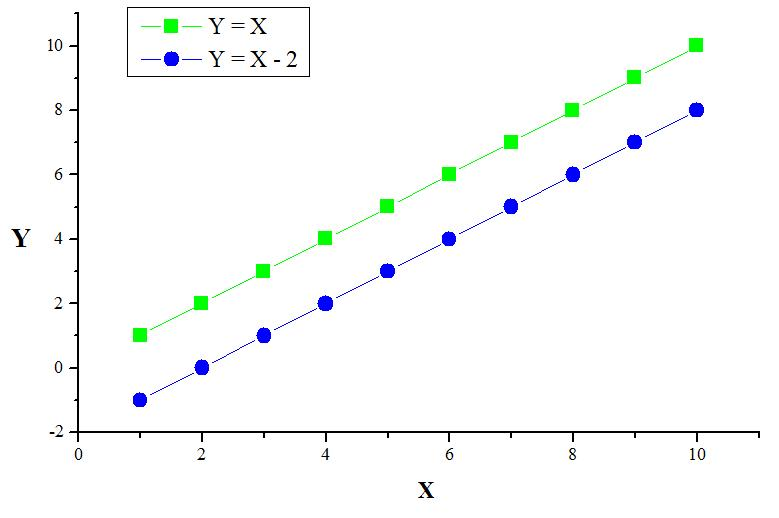
\includegraphics{images/graph.jpg}
}

\caption{
\label{graph-fig}
     Линейные функции.}
\end {center}
\end {figure}
Ссылаемся на график ~\ref{graph-fig}.
Ссылка на статью: \cite{DBLP:conf/adbis/NovikovP03}
\section{Заключение}

%ручной ввод библиографии.
%для тестирования, убрать комментарий
%\begin{thebibliography}{}

%\bibitem{voc} Griffin D.W., Lim J.S. \flqq Multiband excitation vocoder\frqq. IEEE ASSP-36 (8), 1988, pp. 1223-1235.
%\end{thebibliography}

%автоматическая генерация библиографии из бибтеховского файла. Из файла подгрузятся только те статьи, на которые есть ссылки в тексте!
\bibliographystyle{gost780s}
\bibliography{test}

\end{document}
